\chapter{手性：左右手分子并不总是等价}

\begin{kaichang}
请你做两件小事。

第一件：如果有橙子和柠檬，各剥下一小块皮，把果皮朝外对折，闻闻喷出来的那缕雾气。橙子味和柠檬味，你闭着眼也能分清。可如果我告诉你，这两种气味的“主角”是同一种分子——组成相同、原子连接顺序也相同，仅仅互为镜像——你信吗？

第二件：找一只左手的手套，往右手上戴。怎么转手腕都戴不服帖。左手和右手由同样的“零件”组成，骨头、关节一根不少，为什么就是换不了？

把这两个疑问先记在纸上。这一章结束时你会发现：橙皮、手套，还有一场改变了全世界药品监管制度的悲剧，背后是同一条规律——\textbf{镜像，并不总是等价}。
\end{kaichang}

\section{先从一双手套说起}

为什么左手的手套戴不进右手？别急着说“废话”，认真比划一下。把两只手手心朝下叠在一起：指尖对上了，拇指却指向两边；把一只手翻过来让拇指同向，手心手背又对不上了。两只手像照镜子：镜子里外一模一样，却永远无法完全重合。

几何上管这种关系叫“不可叠合的镜像”。生活里这样的东西到处都是：

\begin{itemize}[itemsep=2pt]
\item 螺丝钉的螺纹分左旋和右旋，右旋螺丝顺时针拧紧，左旋螺丝恰好相反——煤气罐的接口故意做成左旋，就是为了让你一眼（一手）摸出它不普通。
\item 大多数田螺的壳是右旋的，左旋的个体极其罕见，被收藏者当成宝贝。
\item 弹簧、螺旋楼梯、牵牛花的藤蔓，都有“绕向”之分，而且绕反了就是另一个东西。
\end{itemize}

这些例子有一个共同点：差别不在“用了什么材料”，而在“材料在三维空间里怎样排列”。左鞋和右鞋用的是同样的皮革和橡胶，差别只存在于空间里。

问题是：分子比手套小上亿倍，我们既看不见也摸不着。凭什么说分子也有“左右手”？这一章的旅程，就是把这只看不见的手套找出来。

\section{把镜头推进：四个不同的邻居}

镜头推进到分子层。回忆第 19 章和第 20 章：碳原子用四根共价键连接伙伴时，四根键不是摊在平面上，而是指向\textbf{四面体}的四个顶点——碳坐在四面体中心，四个邻居各守一个角。

现在做一道填空题。酸奶里的酸味主角乳酸，它正中央的那个碳原子连着四个邻居：一个氢原子（H）、一个羟基（\chem{OH}）、一个甲基（\chem{CH_3}）、一个羧基（\chem{COOH}）。\textbf{四个邻居全都不相同。}

请你在脑子里搭这个模型：中央是碳，四个角随便摆上这四个基团。搭好以后，把其中任意两个基团对调一下位置，得到一个新搭法。问题：新搭法和旧搭法是同一个东西吗？

你可以试着旋转模型——怎么转都没法让它们完全重合，就像怎么转手腕都没法让左手套戴进右手。这两个模型互为镜像，却不可叠合。化学家给这样的分子对起了名字：互为\textbf{对映体}（意思是“成对的镜像”）；中央那个连着四个不同基团的碳，叫做\textbf{手性中心}；分子这种“分左右手”的性质，叫做\textbf{手性}——这个词来自希腊语“手”。

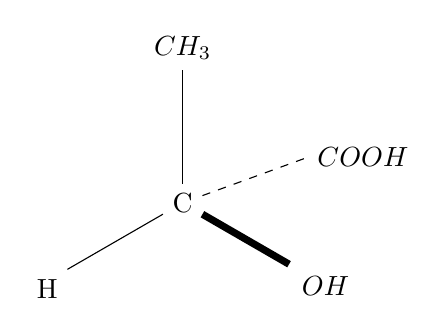
\begin{tikzpicture}[scale=1.3]
  \node (c) at (0,0) {C};
  \draw (c) -- (90:1.3) node[above] {$\chem{CH_3}$};
  \draw (c) -- (210:1.3) node[below left] {H};
  \draw[line width=2.6pt] (c) -- (330:1.2) node[below right] {$\chem{OH}$};
  \draw[dashed] (c) -- (20:1.3) node[right] {$\chem{COOH}$};
\end{tikzpicture}

上面这幅图是化学家画四面体碳的约定：普通细线表示键躺在纸面上，\textbf{加粗的楔形线}表示这根键伸出纸面指向你，\textbf{虚线}表示缩到纸面背后。这只是人为的表示法——分子没有颜色，键也不是小棍子。你不妨用四根牙签插进一块橡皮泥，亲手搭一搭，再把其中两根对调，体会一下“转不回去”的感觉。

先记住三个要点。第一，对映体的组成完全相同，连原子的连接顺序都完全相同，差别只在三维排布。第二，判断一个碳是不是手性中心，只需数它连的四个邻居是否两两不同；只要有任何两个邻居相同（比如乙醇中间的碳连着两个氢），镜像就能叠合，分子就没有手性。第三，手性不是碳的专利，但四面体碳是最常见的手性来源。

\section{普通方法分不开，偏振光却能}

对映体有多像？拿乳酸的两种对映体来说：熔点一样，沸点一样，在水里的溶解度一样，密度一样，跟普通试剂反应的速率也一样。用第 3 章学过的那些分离手段——蒸馏、结晶、过滤——统统分不开它们。这不奇怪：物理性质大多取决于分子的大小、极性、彼此间的吸引力（第 22 章），而镜像的两双手在这些方面分毫不差。

但有一种“光”能分出左右手。

普通的光，振动方向四面八方都有。让光穿过一片偏振片（太阳镜的镜片就是），出来的光只剩一个方向振动，像穿过一排竖直栅栏的绳子波——这叫\textbf{偏振光}。19 世纪初，物理学家发现一件怪事：让偏振光穿过糖水，振动面会被\textbf{拧转}一个角度。溶液仿佛一只看不见的手，把光的振动面拧了拧，而且溶液越浓、光路越长，拧得越多。这种现象叫\textbf{旋光性}。

关键在于：一对对映体，一个把振动面向左拧，另一个向右拧，\textbf{拧的角度一模一样，方向恰好相反}。把两种对映体等比例混在一起，左旋和右旋互相抵消，溶液就“不转”了——这样的混合物叫\textbf{外消旋体}。测量旋光的仪器叫旋光仪，至今仍是药厂质检的常规设备。

\begin{shiyan}
\textbf{在家看“光被拧转”}

材料：一个透明玻璃杯、清水、两勺蜂蜜或玉米糖浆；两片偏振片（旧的不闪式 3D 眼镜镜片、偏振太阳镜都可以）；一部手机或电脑液晶屏。

步骤：把手机屏幕调成纯白图片——液晶屏发出的本来就是偏振光。把一片偏振片挡在眼前看屏幕，慢慢转动镜片，会看到屏幕从亮变到几乎全黑，记下这个位置。然后在镜片和屏幕之间放入装了糖水的杯子（糖水约占三分之一杯，搅匀）。

观察点：原本全黑的屏幕又亮了！把眼前的偏振片再转一个角度，才能重新变黑——你转过的角度，就是糖水把偏振光“拧”过的角度。换清水试试：屏幕保持全黑，因为水分子没有手性。

安全提示：不要隔着镜片直视太阳；玻璃杯轻拿轻放。蜂蜜黏手，做完记得洗手擦桌。
\end{shiyan}

你刚才拧动的那束光，是被糖分子“拧”的。糖分子有手性（第 46 章会细看），而组成蜂蜜的糖清一色是同一只“手”——这一点后面还要回来讲。

\section{巴斯德的镊子}

\begin{zhengju}
分子有左右手这件事，不是谁想出来的，是被一罐晶体逼出来的。故事的主角是 26 岁的法国化学家巴斯德——对，就是后来发明巴氏消毒法的那位，但他的科学生涯是从晶体开始的。

1848 年，巴斯德在研究葡萄酒酿造的副产物酒石酸。当时已知一件怪事：从葡萄酒里直接得到的酒石酸，溶液能让偏振光旋转；而另一种化学成分完全相同、叫做“外消旋酒石酸”的物质，溶液却一点不转。同样的组成，一个转一个不转——已有的理论解释不了。

巴斯德注意到前人留下的一个细节：酒石酸盐的晶体上有些小晶面，只长在晶体的一侧，像手套上的拇指。他猜测：如果分子本身有左右之分，晶体或许也有。于是他取来外消旋酒石酸的钠铵盐溶液，让它在低温下慢慢结晶，然后做了一件事——在显微镜下，用一把镊子，把晶体一颗一颗按晶面朝向分成两堆：晶面朝左的一堆，朝右的一堆。

分别配成溶液送进旋光仪：一堆向左转，一堆向右转，角度相等、方向相反。不转光的“外消旋酒石酸”，原来是两种旋光相反的晶体各一半混起来的！巴斯德后来回忆，他激动得冲出实验室，抱住走廊里遇到的第一个人。

这个故事有三个值得咀嚼的地方。第一，巴斯德的结论不是“我猜分子有手性”，而是可以被检验的预言：两堆晶体必须转出相等而相反的角度——仪器说了算。第二，替代解释也被排除了：如果旋光来自晶体外形而不来自分子，那么晶体溶解后旋光应该消失；事实是溶成溶液照样转，说明手性藏在分子本身。第三，运气也在场：这种盐只在约 $28\,^{\circ}\mathrm{C}$ 以下才结晶成左右分开的两类晶体，温度再高，两种分子就手拉手结成一模一样的晶体，镊子再巧也分不开。巴斯德若在盛夏做实验，历史可能改写。

分子为什么会长成左手右手？1874 年，范托夫和勒贝尔各自独立提出碳的四面体模型，给出了本章开头的那幅图景：四个不同邻居占据四面体四角，镜像不可叠合。当时这被不少人嘲笑为“空想”——谁见过四面体？几十年后 X 射线晶体学直接测出了原子位置，四面体分毫不差。
\end{zhengju}

\section{给左右手起个名字}

到这里，符号终于可以登场了。化学家给对映体定了两套“名字”。

一套按旋光方向：向右转的叫 $(+)$（旧称 d），向左转的叫 $(-)$（旧称 l）。这套名字直观，但只告诉你“光往哪边转”，不告诉你分子的真实排布。

另一套按空间排布本身：给手性中心周围的四个邻居排个优先级，按规则看过去，顺时针的叫 $(R)$（拉丁语“右”），逆时针的叫 $(S)$（拉丁语“左”）。具体规则放进本章的挑战层，主线只需要记住：$(R)$ 和 $(S)$ 描述的是分子的“长相”，跟它把光往哪边转\textbf{没有简单的对应关系}——有的 $(R)$ 分子是 $(+)$，有的 $(R)$ 分子是 $(-)$。把两套名字混为一谈，是初学者最常掉的坑。

于是乳酸可以这样写：$(S)$-$(+)$-乳酸和 $(R)$-$(-)$-乳酸。你运动后肌肉里的乳酸、酸奶里的乳酸，几乎清一色是其中一种；而实验室里用普通化学方法合成的乳酸，却是两种各占一半的外消旋体。为什么生命只造一只手？这正是本章后半段的问题。

\section{鼻子、药片和酶，都能分出左右}

现在可以回答开场的第一问了：既然对映体物理性质一模一样，你的鼻子凭什么分得出橙子和柠檬？

答案藏在“配对”里。请你把手伸进手套——左手套只合左手，右手套只合右手。手套本身是手性的，所以它对“进来的是哪只手”极其挑剔。你的嗅觉受体是蛋白质，而蛋白质（第 48 章细讲）本身就是高度手性的分子机器。当橙皮里的柠檬烯飘进鼻腔，钻进受体这只“手套”时：$(R)$-柠檬烯的形状恰好契合某个受体，你闻到橙子味；它的镜像 $(S)$-柠檬烯塞进去别别扭扭，触发的是另一组受体，你闻到的是柠檬和松木般的气味。\textbf{组成相同，连接相同，只因是镜像，气味就不同}——因为你的鼻子是手性的。

留兰香和葛缕子（西餐和口香糖里常见的香料）也是一对：香气主角香芹酮的两种对映体，一个像薄荷般清凉，一个像茴香籽般辛香。

同样的道理在药片里更严肃。药物分子要起效，通常得嵌进体内某个蛋白质的空腔，像钥匙进锁。锁是手性的，钥匙的镜像自然常常拧不动。常见的止痛药布洛芬，真正抑制炎症的主要是 $(S)$ 型；好在人体里有一套“改装车间”，能把吃下去的一部分 $(R)$ 型慢慢转成 $(S)$ 型，所以药店卖的外消旋布洛芬照样有效——但这也提醒我们，吃下去的镜像分子在体内未必安分。治疗帕金森病的药物左旋多巴，名字里就带着手性：只有“左”的那种能穿过血脑屏障、被神经细胞利用，镜像几乎无效。

酶是挑剔的极致。一把酶做的“锁”往往只认一种手性的底物，镜像递过来，反应速率可能差上千倍甚至完全不反应（第 49 章专门讲酶怎么做到这一切）。也正因如此，药厂生产手性药物时，要么想办法只造出需要的那只“手”，要么造出混合物再费力拆开——这是现代制药工业成本的大头之一。

\section{沙利度胺：一个必须讲完整的故事}

手性课上几乎必讲沙利度胺（商品名“反应停”），但这个故事常被压缩成一句“右手分子是良药，左手分子是毒药，后来禁了左手分子就天下太平”。真实的历史要曲折得多，也更有教益。我们慢慢讲。

1957 年，西德格兰泰公司把沙利度胺作为镇静剂推向市场，宣称它安全到“孕妇都能吃”，很快在几十个国家作为缓解孕吐的非处方药热销。注意当时的监管背景：多数国家只要求药厂自证“吃不死人”，\textbf{不要求检验对孕妇和胎儿的影响}，也不要求证明药物真的有效。动物实验做得潦草，孕期用药干脆没人试过。

美国是个例外，但例外得偶然。按照 1938 年的法律，新药上市需经食品药品监督管理局（FDA）审查安全性。审批员弗朗西丝·凯尔西拿到申请材料后，认为安全证据单薄——尤其缺少孕期和长期用药的数据——顶住药厂一次次催促，迟迟不批。从 1960 年到 1961 年，沙利度胺始终没能进入美国市场。

1961 年，德国医生伦茨和澳大利亚医生麦克布赖德先后发出警报：一种罕见的出生缺陷（四肢短小如鳍状的“海豹肢症”）突然成批出现，时间线与母亲孕早期服用沙利度胺高度吻合。当年年底，药物在各国陆续撤市。全球约有上万名婴儿因此带着终身残疾出生；美国因为凯尔西的拖延，受害病例极少。第二年，美国国会通过修正案，从此新药上市必须同时证明\textbf{安全且有效}，药物上市后的不良反应监测制度也在各国逐步建立。这场悲剧塑造了我们今天的药品监管体系。

现在讲立体化学，而且要讲全。沙利度胺分子确实有一个手性中心。动物研究显示，$(S)$ 型与胎儿发育的损害关联更强——2010 年，科学家找到了它的分子靶点：一种叫 cereblon 的蛋白质，$(S)$ 型与它结合得更牢。看到这里，那句流行口诀似乎成立？

不。两个被流行版本省掉的事实才是关键。第一，沙利度胺的两种对映体在体温、血液酸碱度的条件下会\textbf{快速互相转变}，几小时内就变成对半开的外消旋体。也就是说，就算当年药厂只卖“纯净的 $(R)$ 型”，病人吃进去几小时后，体内照样出现大量 $(S)$ 型。第二，更细致的研究表明两种对映体的药理作用本就互相交叠，并非一个全善一个全恶。把悲剧简化为“坏手性惹的祸”，既不符合化学事实，也掩盖了真正的教训——\textbf{真正的漏洞在于监管没要求孕期证据、在于“安全”的宣称没有证据支撑}。凯尔西挡住的恰恰不是“坏的那一半分子”，而是整盒没经过检验的药。

故事的尾声同样反直觉：沙利度胺并没有被扫进历史的垃圾堆。1964 年，一位医生用它治疗麻风病人的一种严重炎症并发症，效果惊人；1998 年，FDA 在附带极严格管控（育龄患者强制避孕、处方登记追踪）的条件下重新批准了它，如今它还是治疗多发性骨髓瘤的重要药物之一。同一种分子，对一种用途是灾难，对另一种用途是良药——决定结果的是证据、剂量、适用人群和监管，而不是分子标签上的“好”与“坏”。

\begin{qiaoliang}
“只要分子足够纯，就不会有另一种手性混进来”——用数字戳破这个直觉。

一片 100 mg 的沙利度胺含多少个分子？它的摩尔质量约 \ud{258}{g\cdot mol^{-1}}，所以 0.1 g 药约含 $0.1\div258\approx3.9\times10^{-4}$ mol，乘以阿伏伽德罗常数 \ud{6.02\times10^{23}}{mol^{-1}}（第 5 章），得到约 $2.3\times10^{20}$ 个分子——两千亿亿个。

假设药厂把纯度做到了惊人的 99.99\%，即每万个分子里只有一个是“镜像杂质”。算一算：$2.3\times10^{20}\times0.0001=2.3\times10^{16}$——\textbf{仍有上千万亿个}镜像分子。这还没算进入人体后的互相转变。化学家追求高纯度当然有意义，但“绝对纯净的一只手”在分子世界里是不存在的；真正保护病人的，是把证据标准和监测体系做到位。
\end{qiaoliang}

\section{生命为什么清一色“左撇子”}

把五个贯穿问题中的最后一个摆上台面：手性在生命中怎样被保存、复制、调节和选择？

请看一份惊人的清单。组成你全身蛋白质的氨基酸，几乎清一色是同一种手性（称为 L 型）；你 DNA 里的糖，清一色是另一种手性（称为 D 型）。不是 99\%，是接近 100\%——地球上几十亿种生物，从细菌到蓝鲸，全部遵守同一套“手性宪法”。这套规则一代代复制至今，几十亿年没变过。

为什么非如此不可？想想蛋白质：它是一条氨基酸链折叠成的精密机器（第 48 章），如果链上左手右手零件混着用，折叠出来的形状就乱了套，机器直接报废。手套的道理再次登场：整条流水线必须用同一套模具。

那为什么偏偏是 L 型氨基酸、D 型糖，而不是反过来？坦白说：\textbf{还不知道}。有证据供你参考：落在地球上的某些陨石里，几种氨基酸的 L 型略微多于 D 型，说明太空里的化学过程就能制造微小的“手性倾斜”；实验室里也发现过能自我放大的反应——产物稍稍偏向一只手，这只手就会催化生成更多自己，把小倾斜滚成大雪球。物理学家还指出，自然界四种基本力之一的弱相互作用本身就分左右，给两种镜像造成极其微小的能量差。这些线索都真实存在，但哪条是主因、它们怎样串成完整因果链，至今没有公认的答案。科学还没交卷的问题，恰恰是科学活着的证据——第 87 章我们还会回到这类悬案。

\section{这个模型什么时候会失灵}

“四个不同邻居的碳产生手性”是个强大的模型，但知道它在哪里失灵，才算真正掌握。

\begin{itemize}[itemsep=2pt]
\item \textbf{有手性中心，分子却可能没有手性}。酒石酸分子有两个手性中心，但它有一种形态：两个中心的“拧法”恰好相反，分子内部存在对称面，像一个人左手戴右手套、右手戴左手套——整体竟然能和自己的镜像叠合！这种“内消旋体”不旋光。巴斯德当年研究的酒石酸家族，正是靠这个第三条路线凑齐了所有可能性。
\item \textbf{没有手性中心，分子也可能有手性}。丙二烯类分子两端的取代基互相垂直，整个分子像拧过的毛巾，照样分左右；某些螺旋形分子本身就是一道螺旋。
\item \textbf{手性中心会被“拆掉”}。沙利度胺的教训正在于此：只要手性中心上存在一条化学上可行的“翻转通道”，两种镜像就会自动对半混合，时间尺度从几秒到几小时不等。判断一个分子“能不能保持自己的手”，不能只看结构图，还要看它在真实环境里的化学。
\item \textbf{对映体的差异只在手性环境里显现}。在非手性的世界——普通溶剂、普通试剂、普通物理测量——两只手表现完全一致。差异是在遇到另一只“手”（偏振光、手性受体、酶）的瞬间才冒出来的。所以“镜像分子性质相同”这句话，在真空里成立，在你的身体里不成立。
\end{itemize}

\begin{wuqu}
“对映体嘛，除了让偏振光转的方向相反，其他性质全都一样。”

反例一：香芹酮的两种对映体，一个闻起来像留兰香薄荷，一个像葛缕子籽——气味不同，说明它们与你鼻腔受体的结合不同。反例二：左旋多巴有效，它的镜像几乎无效。反例三：酶往往只催化其中一种对映体，速率相差成百上千倍。

正确的说法是：对映体在\textbf{非手性环境}中的物理化学性质相同（熔点、沸点、普通溶解度），一旦进入\textbf{手性环境}（偏振光、手性受体、酶、手性催化剂），差别就可能大到决定生死。你的生命本身就是最挑剔的手性环境。
\end{wuqu}

\section{回到橙皮、柠檬和手套}

现在兑现开场的承诺。

橙皮喷出的雾气里，主角是 $(R)$-柠檬烯；柠檬皮和松节油里，主角是它的镜像 $(S)$-柠檬烯。两种分子的原子组成、连接顺序完全相同，物理性质难分彼此，但你的嗅觉受体是一群手性的蛋白质“手套”，两只手伸进来，握感不同，于是你闻出了橙子和柠檬。闭着眼分得清两种果香的你，其实在做一台精密的手性识别实验。

至于那只戴不进去的手套：左手和右手由同样的零件组成，只因三维排布互为镜像而不可互换——分子世界的乳酸、柠檬烯、沙利度胺，遵循的是同一条几何学。你手上的困惑和鼻腔里的香气，隔着尺度遥相呼应。

还有开场没点破的第三件事：一场改变世界的药品悲剧。沙利度胺的镜像差别是真的，但真正的教训不是“左手分子有毒”，而是：当化学的复杂性（体内互变、靶点结合）遇上缺位的证据标准，受害的永远是证据链条最薄弱处的人——当时是还没来得及出生的胎儿。

\section{把“只造一只手”变成工业}

理解手性不是为了欣赏灾难，而是为了掌握它。今天的制药工业有两件法宝。

第一件叫\textbf{不对称催化}：既然普通合成总是造出左右各半的外消旋体，那就让催化剂本身带上手性——反应在“手性的模子”里进行，产物天然偏向一只手。2001 年的诺贝尔化学奖就颁给了这条路的开创者：诺尔斯用它实现了左旋多巴的工业化生产，野依良治把效率推到工业可用的高度，沙普利斯则让一大类氧化反应“只出一只手”。薄荷醇、抗生素、降压药，今天许多药物都是靠手性催化或手性拆分（用色谱柱把两种镜像分开）做出来的。

第二件是监管的遗产：手性药物的审批如今要求把两种对映体各自的吸收、转化、毒理分别查清——这正是沙利度胺事件刻在制度里的碑文。

不过，故事到这里露出了更大的悬念。我们已经知道：你的受体是手性的，你的酶是手性的，你的 DNA 和蛋白质全部只用一种手性的零件。那么——这些零件本身是什么？蛋白质凭什么折叠成只认一只手的“手套”？酶又怎样在毫秒之间完成识别？下一篇我们就要跨过那道门槛：从“分子怎样排列”走进“分子怎样组成生命”。构成你的二十种氨基酸即将登场（第 46 章先讲糖，第 48 章讲蛋白质，第 49 章讲酶），它们每一个都带着今天认识的那只“手”。

\begin{tiaozhan}
$(R)$ 和 $(S)$ 到底是怎么定出来的？规则叫 CIP 次序规则，分三步。第一步：给手性中心连的四个基团排序，直接相连的原子原子序数大者排前（比如 \chem{OH} 的氧 $>$ \chem{COOH} 的碳 $>$ \chem{CH_3} 的碳 $>$ H）；打平就看下一层原子，逐级外推。第二步：把排序最低的那个基团转到背离你的方向（想象它插进纸面）。第三步：看剩下三个基团从高到低的走向——顺时针为 $(R)$，逆时针为 $(S)$。

拿乳酸练手：四个邻居排序为 \chem{OH} $>$ \chem{COOH} $>$ \chem{CH_3} $>$ H。让 H 朝后，若 \chem{OH} $\rightarrow$ \chem{COOH} $\rightarrow$ \chem{CH_3} 是逆时针，就是 $(S)$ 型——你肌肉里的乳酸正是它。注意一个反直觉的事实：这套规则是纯粹的人为约定，和分子把偏振光往哪边转毫无公式上的联系。$(S)$-乳酸是 $(+)$ 的，而有些 $(S)$ 分子是 $(-)$ 的。命名归命名，旋光归旋光——这正是科学约定“先定义清楚再使用”的范例。跳过本框不影响主线。
\end{tiaozhan}

\section*{练一练}

\begin{sikaoti}
\item 用牙签和橡皮泥（或纸笔仿照本章的楔形—虚线约定）画出乳酸的两种对映体，标出手性中心。试着在纸上把其中一个旋转几次，说明为什么无论怎样旋转都无法与另一个完全重合。图旁注明：这是帮助思考的表示法，真实的键不是小棍。
\item 下列分子里，哪些碳是手性中心？乙醇（\chem{CH_3CH_2OH}）、乳酸（\chem{CH_3CH(OH)COOH}）、甘油（\chem{HOCH_2CH(OH)CH_2OH}）。逐个说出你数“四个邻居”的过程。
\item 画一张本章家庭实验的光路示意图：液晶屏、糖水杯、偏振片，标出每一步光的偏振方向发生了什么变化，并解释为什么把糖水换成清水后屏幕保持全黑。
\item 外消旋体是两种对映体等量的混合物，单个分子明明都会旋光，为什么整杯溶液测不出旋光？用“每个分子都在拧光”的图景解释这种抵消。
\item 酒石酸有两个手性中心。一种形态是内消旋体，不旋光。请用文字或简图说明：为什么“有手性中心”不保证“分子有手性”？（提示：想想那个左手戴右手套、右手戴左手套的人。）
\item 一位药厂发言人宣称：“我们的新工艺能生产出 100\% 纯净的 $(R)$ 型沙利度胺，因此绝对安全。”请用本章的两个事实反驳他，并说明真正应该补上的是什么。
\end{sikaoti}
